\documentclass{article}

% Language Setting
\usepackage[english]{babel}

% Set page size and margins
\usepackage[letterpaper,top=2cm,bottom=2cm,left=3cm,right=3cm,marginparwidth=1.75cm]{geometry}

% Useful packages
\usepackage{amsmath}
\usepackage{graphicx}
\usepackage{listings}
\usepackage[colorlinks=true, allcolors=blue]{hyperref}

\title{Question 27: Conical Paper Cup Problem}
\author{Alec Him}
\date{}

\begin{document}
\maketitle


\section{Introduction}
This document contains the mathematical derivation and calculations for solving the Conical Paper Cup Problem. The goal is to maximize the volume of the conical cup formed by removing a sector of length \( x \) from a circular waxed paper of radius \( R \).
\begin{figure}[h!]
    \centering
    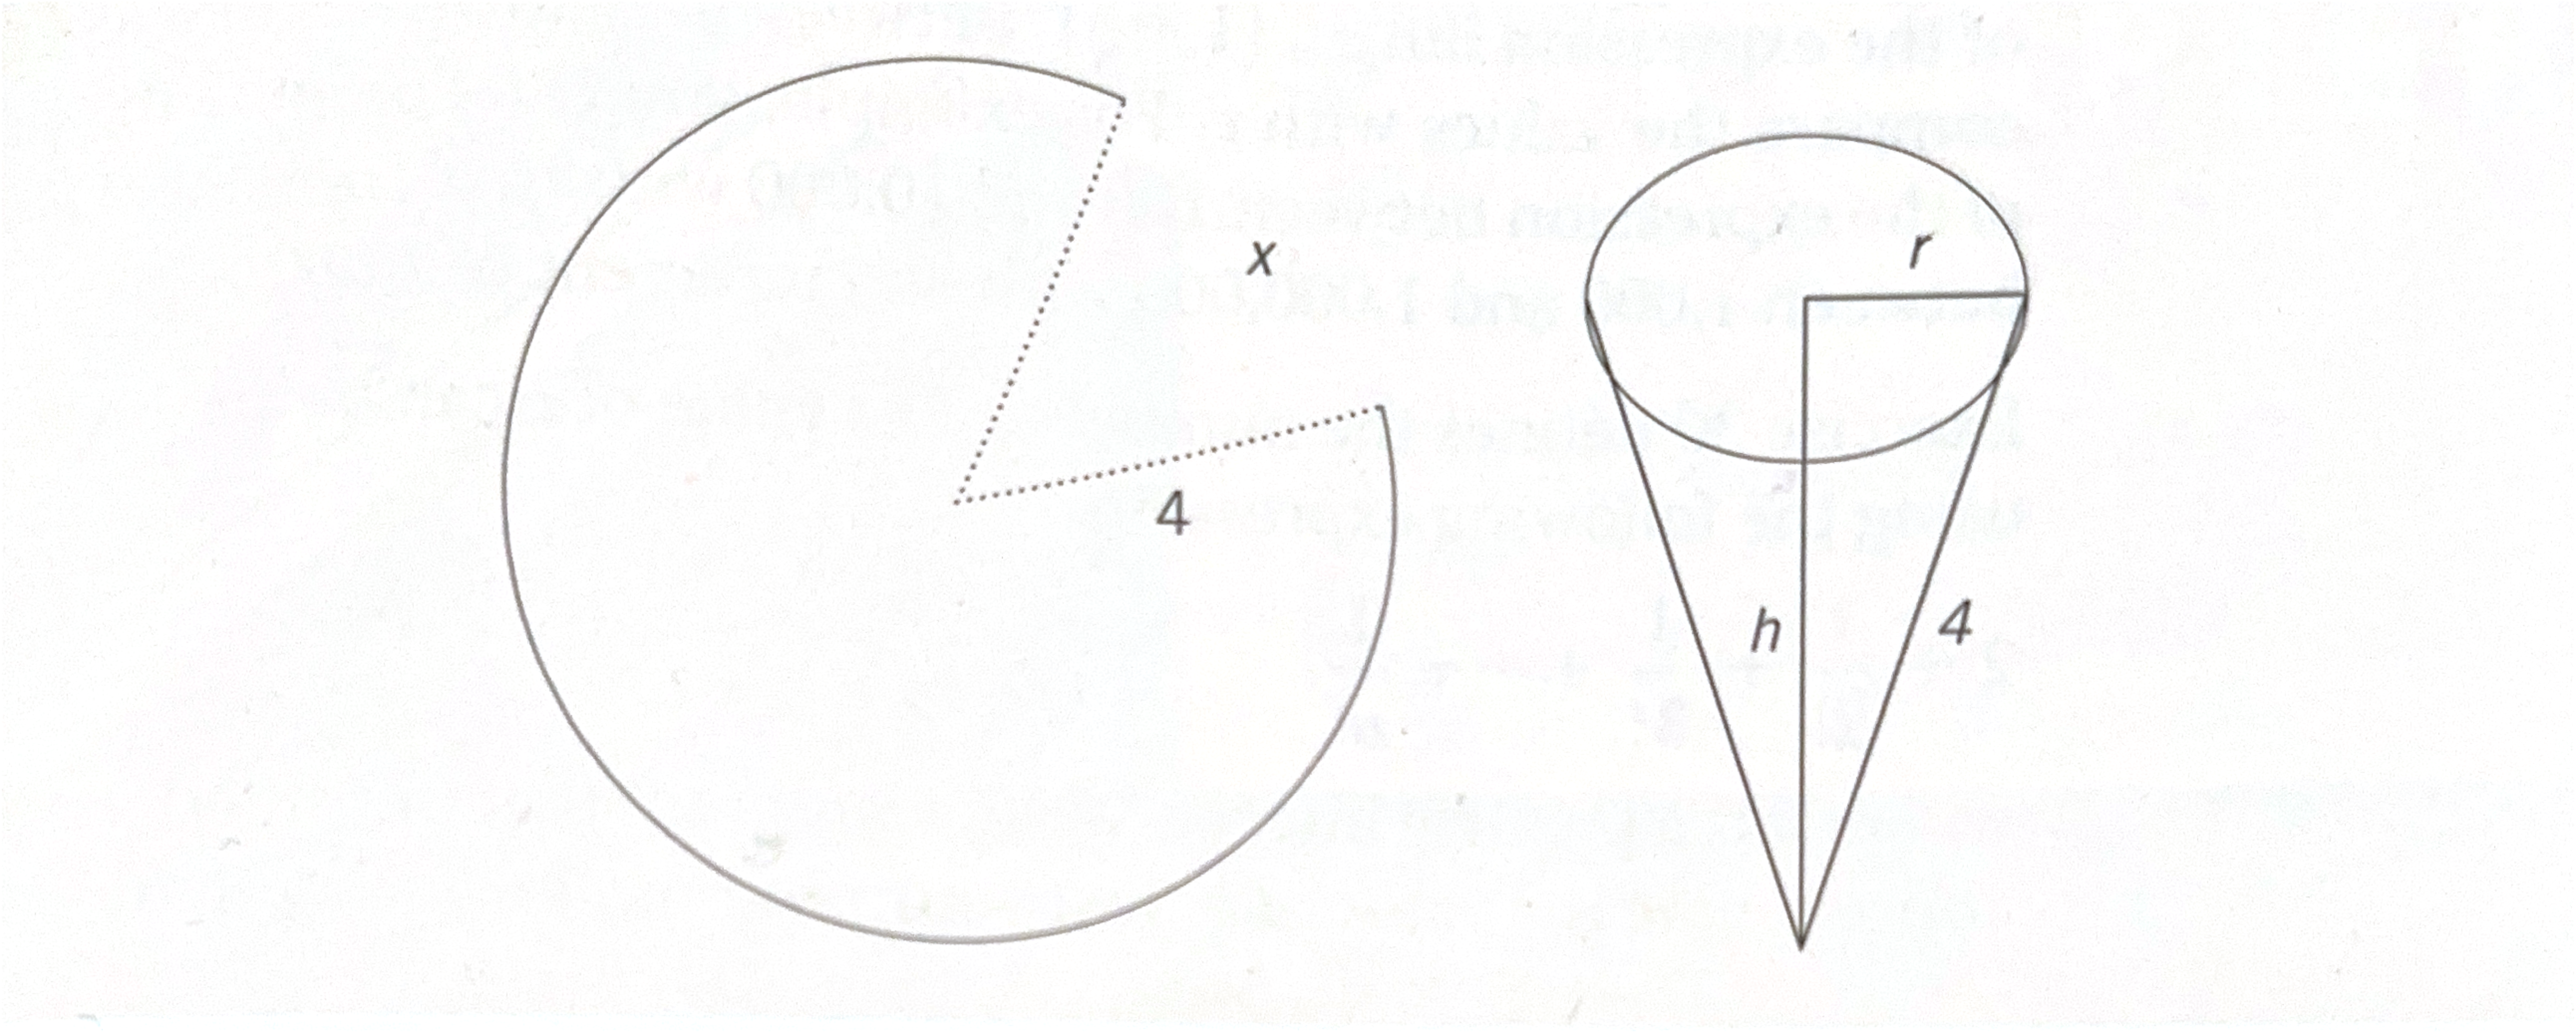
\includegraphics[width=0.6\textwidth]{Figure1.pdf}
    \caption{Diagram of the conical paper cup problem showing a circle (radius 4), cut arc (x), and inscribed cone (height h, radius r).}
    \label{fig.Graph}
\end{figure}


\section{Variables}
\begin{itemize}
    \item \( R \) : Radius of the circular waxed paper (user inputted as \texttt{circleRadius}).
    \item \( r \) : Base radius of the resulting cone.
    \item \( h \) : Height of the resulting cone.
    \item \( s \) : Slant height of the cone, which is equal to \( R \) (since the remaining sector's arc forms the cone's circumference).
    \item \( x \) : Length of the removed sector.
\end{itemize}


\section{Formulation and Derivation}
When a sector of length is removed, the remaining arc length becomes:
\begin{equation}
    2\pi R - x
\end{equation}
This arc forms the circumference of the base of the resulting cone, so:
\begin{equation}
    2\pi r = 2\pi R - x
\end{equation}
Solving for \( r \):
\begin{equation}
    r = \frac{2\pi R - x}{2\pi}
\end{equation}
Using the Pythagorean theorem, since the slant height is \( R \):
\begin{equation}
    h = \sqrt{R^2 - r^2}
\end{equation}
The volume of the cone is given by:
\begin{equation}
    V = \frac{1}{3} \pi r^2 h
\end{equation}
Substituting \(r = \frac{2\pi R - x}{2\pi} \) and \(h = \sqrt{R^2 - r^2} \):
\begin{equation}
    V = \frac{1}{3} \pi \left(\frac{2\pi R - x}{2\pi}\right)^2 \sqrt{R^2 - \left(\frac{2\pi R - x}{2\pi}\right)^2}
\end{equation}


\section{Maximization using Calculus}
To maximize \( V \), differentiate \( V \) with respect to \( x \) and set \( \frac{dV}{dX} = 0 \).
\begin{equation}
    \frac{dV}{dx} = \frac{d}{dx} \left[\frac{1}{3} \pi \left(\frac{2\pi R - x}{2\pi}\right)^2 \sqrt{R^2 - \left(\frac{2\pi R - x}{2\pi}\right)^2} \right] = 0
\end{equation}
\subsection{Define \( u \) and \( v \)}
Let \( u = \left(\frac{2\pi R - x}{2\pi}\right)^2 \) and \( v = \sqrt{R^2 - \left(\frac{2\pi R - x}{2\pi}\right)^2} \). \\ \\
\noindent Then: 
\begin{equation}
    V(x) = \frac{\pi}{3} * u * v
\end{equation}
Using the product rule:
\begin{equation}
    V'(x) = \frac{\pi}{3}\left(u'v+uv'\right)
\end{equation}
where \( u' \) and \( v' \) are derivatives of u and v.


\subsection{Differentiate \( u' \)}
\begin{displaymath}
    u = \left(\frac{2\pi R - x}{2\pi}\right)^2 = (r)^2
\end{displaymath}
Using the chain rule:
\begin{align*}
    \frac{du}{dx}\left[\left(\frac{2\pi R - x}{2\pi}\right)^2\right] &= 2\left(\frac{2\pi R - x}{2\pi}\right) * \frac{d}{dx}\left(\frac{2\pi R - x}{2\pi}\right) \\
    &= 2\left(\frac{2\pi R - x}{2\pi}\right) * \left(-\frac{1}{2\pi}\right) \\
    &= -\frac{2\pi R - x}{2\pi^2}
\end{align*}
So we have:
\begin{displaymath}
    u' = -\frac{2\pi R - x}{2\pi^2}
\end{displaymath}


\subsection{Differentiate \( v' \)}
\begin{displaymath}
    v = \sqrt{R^2 - \left(\frac{2\pi R - x}{2\pi}\right)^2} = \sqrt{R^2 - r^2}
\end{displaymath}

\noindent Using the chain rule:
\begin{align*}
    \frac{dv}{dx}\left[\sqrt{R^2 - r^2}\right] 
    &= \frac{1}{2 \sqrt{R^2 - r^2}} * \frac{d}{dx}\left(R^2 - r^2\right) \\
    &= \frac{1}{2 \sqrt{R^2 - r^2}} * \frac{d}{dx}\left(R^2 - u\right) \\
    &= \frac{1}{2 \sqrt{R^2 - r^2}} * \left( -u' \right) \\
    &= \frac{1}{2 \sqrt{R^2 - r^2}} * \left( \frac{2\pi R - x}{2 \pi^2} \right) \\
    &= \frac{2\pi R - x}{4\pi^2 \sqrt{R^2 - r^2}}
\end{align*}
So we have:
\begin{displaymath}
    v' = \frac{2\pi R - x}{4\pi^2 \sqrt{R^2 - r^2}}
\end{displaymath}

\subsection{Applying the Product Rule for \( V(x) \)}
Using the product rule: 
\begin{displaymath}
    V'(x) = \frac{\pi}{3}\left(u'v+uv'\right)
\end{displaymath}
Substituting \( u' \) and \( v' \):
\begin{displaymath}
    V'(x) = \frac{\pi}{3}\left[\left(-\frac{2\pi R - x}{2\pi^2}\right) * \sqrt{R^2 - r^2} + \left(\frac{2\pi R - x}{2\pi}\right)^2 * \frac{2\pi R - x}{4\pi^2\sqrt{R^2 - r^2}}\right]
\end{displaymath}


\section{Maximum Volume}
Set V'(x) = 0:
\begin{displaymath}
    V'(x) = \frac{\pi}{3}\left[\left(-\frac{2\pi R - x}{2\pi^2}\right) * \sqrt{R^2 - r^2} + \left(\frac{2\pi R - x}{2\pi}\right)^2 * \frac{2\pi R - x}{4\pi^2\sqrt{R^2 - r^2}}\right]
\end{displaymath}
Expand Equation:
\begin{align*}
    \frac{\pi}{3}*\left(2\pi R - x\right)\left[\left(\frac{\sqrt{R^2 - r^2}}{2\pi^2}\right) + \left(\frac{4\pi^2 R^2 - x^2}{16\pi^4 \sqrt{R^2 - r^2}}\right)\right] = 0 \\
    \frac{\pi}{3}*\left(2\pi R - x\right)\left(\frac{\left(8\pi^2 * \left(R^2 - r^2\right)\right) + 4\pi^2 R^2 - x^2}{16\pi^4 \sqrt{R^2 - r^2}}\right) = 0 
\end{align*}
We can remove \( \frac{\pi}{3} * (2\pi R - x) \) and solve within the brackets:
\begin{align*}
    \frac{8\pi^2 * \left(R^2 - \left(\frac{2\pi R - x}{2\pi}\right)^2\right) + 4\pi^2 R^2 - x^2}{16\pi^4 \sqrt{R^2 - \left(\frac{2\pi R - x}{2\pi}\right)^2}} &= 0 \\
    \frac{8\pi^2 * \left(R^2 - \left(R^2 - \frac{x^2}{4\pi^2}\right)\right) + 4\pi^2 R^2 - x^2}{16\pi^4 \sqrt{R^2 - \left(R^2 - \frac{x^2}{4\pi^2}\right)}} &= 0 \\
    \frac{8\pi^2 * \left(- \frac{x^2}{4\pi^2}\right) + 4\pi^2 R^2 - x^2}{16\pi^4 \sqrt{- \frac{x^2}{4\pi^2}}} &= 0 \\
    \frac{8\pi^2 * \left(- \frac{x^2}{4\pi^2}\right) + 4\pi^2 R^2 - x^2}{16\pi^4 - \frac{x}{2\pi}} &= 0 \\
\end{align*}
\begin{align*}
    \frac{-2x^2 + 4\pi^2 R^2 - x^2}{\frac{32\pi^5 - x}{2\pi}} &= 0 \\
    \frac{-3x^2 + 4\pi^2 R^2}{\frac{32\pi^5 - x}{2\pi}} &= 0 \\
    \frac{-6\pi x^2 + 8\pi^3 R^2}{32\pi^5 - x} &= 0
\end{align*}
Since this equals zero and assuming the denominator is not zero, we can focus on the numerator:
\begin{align*}
    -6\pi x^2 + 8\pi^3 R^2 &= 0 \\
    -6\pi x^2 &= -8\pi^3 R^2 \\
    x^2 &= \frac{8\pi^3 R^2}{6\pi} \\
    x^2 &= \frac{4\pi^2 R^2}{3} \\
    x &= \sqrt{\frac{4\pi^2}{3}} * R
\end{align*}

\section{Conclusion}
The solution \( x = R\sqrt{\frac{4\pi^2}{3}} \) represents the optimal cut length that maximizes the cone's volume. We can verify this solution by examining boundary conditions: 
\begin{itemize}
    \item When \( x = 0 \), no sector is removed, resulting in a flat disc with zero volume. 
    \item When \( x = 2\pi R \), we remove the entire circumference, again resulting in zero volume. 
\end{itemize}
Our solution falls between these two extremes.

\end{document}